\documentclass[aspectratio=169,
hyperref={colorlinks,urlcolor=blue}
]{beamer}


%\usetheme{Pittsburgh}
\usetheme{default}
\usepackage{colortbl}%colored tables
%For using helvetica font:
\usepackage[scaled]{helvet}
\usepackage[T1]{fontenc}
\renewcommand\familydefault{\sfdefault}
\urlstyle{same} %sets the fonts for urls
\usepackage{pdfpages}
\usepackage{siunitx}
\usepackage{caption}
\usepackage{pifont}%for dings
\usepackage{pgfplots}%for 3d plotting
\pgfplotsset{compat = newest}
\usepackage{mathtools}%box in align env \Aboxed
\usepackage[american,smartlabels]{circuitikz}%for drawing circuits
\usepackage{multimedia}
\usepackage{animate}
\usepackage{xcolor}


\usetikzlibrary{arrows}
\usetikzlibrary {3d} 
\usetikzlibrary{decorations.markings, math}
\usetikzlibrary{intersections, pgfplots.fillbetween}
\usetikzlibrary {shapes.geometric} 


%\definecolor{myblue}{RGB}{5, 34, 150}
\definecolor{myblue2}{RGB}{5, 34, 150}
\definecolor{myblue}{RGB}{0,36,82}
\definecolor{myred}{RGB}{207, 2, 13}
\definecolor{mygreen}{RGB}{0, 158, 11}
\definecolor{myyellow}{RGB}{220,220,0}
\definecolor{qblue}{RGB}{0,36,82}
\definecolor{qgold}{RGB}{250,189,15}
\definecolor{qred}{RGB}{185,14,49}
\definecolor{cblue}{rgb}{0.13, 0.67, 0.8}
\definecolor{corange}{rgb}{0.8, 0.34, 0.0}
\definecolor{cpurple}{rgb}{0.54, 0.29, 0.42}

%%%%%%%%%%%% General settings
\setbeamercolor{frametitle}{fg=black}
\setbeamercolor{title}{fg=black}
\setbeamercolor{author}{fg=myblue2}

\beamertemplatenavigationsymbolsempty %no navigation controls at bottom of slides
%\setbeamertemplate{footline}[frame number]
\usefonttheme{professionalfonts} 
\setbeamerfont{title}{series=\bfseries,parent=structure}
\setbeamerfont{frametitle}{series=\bfseries,parent=structure}

%%%%%%%%%%%%Lists
\setbeamertemplate{itemize item}[circle] %{\color{myblue}$\circ$}
\setbeamertemplate{itemize subitem}{\color{myblue2}$\circ$}
\setbeamertemplate{itemize subsubitem}{\color{myblue2}$\cdot$}
\setbeamercolor{itemize item}{bg=myblue2,fg=myblue2}
\setbeamercolor{enumerate item}{bg=myblue2,fg=myblue2}
%%%%%%%%%%%%%%%%%%%%%%%%%%%%

%%%%%%%%%%%%Blocks
\setbeamertemplate{blocks}[rounded]
%Default block
\setbeamercolor{block title}{bg=myblue2, fg=white}
\setbeamercolor{block body}{bg=myblue2!10}
\setbeamerfont{block body}{size=\scriptsize}
\setbeamerfont{block title}{size=\scriptsize}
%Alert block
\setbeamercolor{block title alerted}{bg= myblue2, fg=white}
\setbeamercolor{block body alerted}{bg=myblue2!10}
\setbeamerfont{block body alerted}{size=\scriptsize}
\setbeamerfont{block title alerted}{size=\scriptsize}
%example block
\setbeamercolor{block title example}{bg=mygreen, fg=white}
\setbeamercolor{block body example}{bg=mygreen!10}
\setbeamerfont{block body example}{size=\scriptsize}
\setbeamerfont{block title example}{size=\scriptsize}
%%%%%%%%%%%%%%%%55


%%%%%%%%%%%%Figures and captions
\captionsetup{font=scriptsize,labelfont=scriptsize}
%\setbeamertemplate{caption}{\raggedright\insertcaption\par}
\newenvironment{capfig}[3]{\begin{figure}\includegraphics[width=#1\textwidth]{#2}\caption*{\textit{#3}}\end{figure}}{}

%\makeatother
%\setbeamertemplate{footline}
%{
%  \leavevmode%
%  \hbox{%
%  \begin{beamercolorbox}[wd=.4\paperwidth,ht=2.25ex,dp=1ex,center]{author in head/foot}%
%    \usebeamerfont{author in head/foot}\insertshortauthor
%  \end{beamercolorbox}%
%  \begin{beamercolorbox}[wd=.6\paperwidth,ht=2.25ex,dp=1ex,center]{title in head/foot}%
%    \usebeamerfont{title in head/foot}\insertshorttitle\hspace*{3em}
%    \insertframenumber{} / \inserttotalframenumber\hspace*{1ex}
%  \end{beamercolorbox}
%  }%
%  \vskip0pt%
%}
%\makeatletter

\makeatother
\setbeamertemplate{footline}
{
  \leavevmode%
  \hbox{%
\begin{beamercolorbox}[wd=.27\paperwidth,ht=2.25ex,dp=1ex,center]{author in head/foot}%
    \color{black}{\insertinstitute}
\end{beamercolorbox}
  \begin{beamercolorbox}[wd=.27\paperwidth,ht=2.25ex,dp=1ex,center]{author in head/foot}%
    \color{black}{\inserttitle}
  \end{beamercolorbox}%
  \begin{beamercolorbox}[wd=.27\paperwidth,ht=2.25ex,dp=1ex,center]{title in head/foot}%
    \color{black}{\insertshortauthor}
  \end{beamercolorbox}
  \begin{beamercolorbox}[wd=.27\paperwidth,ht=2.25ex,dp=1ex,center]{title in head/foot}%
    \hspace{.28\paperwidth}\color{black} \insertframenumber{} / \inserttotalframenumber\hspace*{1ex}
  \end{beamercolorbox}
  }%
  \vskip0pt%
}
\makeatletter

\setbeamertemplate{title page}
{
  \begin{tikzpicture}[remember picture,overlay]
    \def\barh{4}%15
  
    \draw[color=myblue2,line width=\barh] ([yshift=-0.5*\barh]current page.north west) -- ([yshift=-0.5*\barh,xshift=-0.67\paperwidth]current page.north east);
    \draw[color=myblue2,line width=\barh] ([yshift=-0.5*\barh,xshift=-0.67\paperwidth]current page.north east) -- ([yshift=-0.5*\barh,xshift=-0.34\paperwidth]current page.north east);
    \draw[color=myblue2,line width=\barh] ([yshift=-0.5*\barh,xshift=-0.34\paperwidth]current page.north east) -- ([yshift=-0.5*\barh]current page.north east); 
  
    \draw[color=myblue2,line width=\barh] ([yshift=0.5*\barh]current page.south west) -- ([yshift=0.5*\barh,xshift=-0.67\paperwidth]current page.south east);
    \draw[color=myblue2,line width=\barh] ([yshift=0.5*\barh,xshift=-0.67\paperwidth]current page.south east) -- ([yshift=0.5*\barh,xshift=-0.34\paperwidth]current page.south east);
    \draw[color=myblue2,line width=\barh] ([yshift=0.5*\barh,xshift=-0.34\paperwidth]current page.south east) -- ([yshift=0.5*\barh]current page.south east);
    %\node[left] at (current page.east) {
    %
\includegraphics[scale=0.1]{figures/coverpage}
    %};
  \end{tikzpicture}
  
  \usebeamerfont{title}\usebeamercolor[fg]{title}\inserttitle\par
  \usebeamerfont{subtitle}\usebeamercolor[fg]{subtitle}\insertsubtitle\par
  \vspace{2cm}
  \usebeamerfont{author}\usebeamercolor[fg]{author}\insertauthor\par
  \usebeamerfont{institute}\usebeamercolor[fg]{author}\insertinstitute\par
  \usebeamercolor[fg]{author}\par
  \usebeamercolor[fg]{titlegraphic}\inserttitlegraphic

} 

\setbeamertemplate{frametitle}{%
    \nointerlineskip%
        \par\hspace*{-\dimexpr0.5\paperwidth-0.5\textwidth}\textcolor{myblue2}{\rule{0.33\paperwidth}{6pt}}\textcolor{myblue2}{\rule{0.33\paperwidth}{6pt}}\textcolor{myblue2}{\rule{0.34\paperwidth}{6pt}} 
    \begin{beamercolorbox}[wd=\paperwidth,ht=0.75cm,dp=0.6ex]{frametitle}
        \hspace*{0.5cm}\strut\usebeamerfont{frametitle}\insertframetitle\strut
        %\hrule
    \end{beamercolorbox}%
    %%Line below:
%\par\hspace*{-\dimexpr0.5\paperwidth-0.5\textwidth}\textcolor{myblue}{\rule{\paperwidth}{0.4pt}}
     % <-- calculation of left margin width + rule
     %\textcolor{red}{\noindent\rule{\paperwidth}{2pt}}
}


%%%%%%%%%%%%Frame templates

%Slide with title
\newenvironment{titleframe}[1]
{\begin{frame}\frametitle{#1}\end{frame}}
{}

%Slide with title and itemize list:
\newenvironment{bulletframe}[1]
{\begin{frame}{#1} \itemize}
{\enditemize \end{frame}}

%Slide with two columns 50/50
\newenvironment{twocolframe}[3]
{\begin{frame}{#1}
 \begin{columns}[T]
 \column{0.5\textwidth}#2
 \column{0.5\textwidth}#3
 \end{columns}\end{frame}}{}

%Slide with two columns 60/40 <<<<<<<<<<<<<<<<<<<<<<  This one!
\newenvironment{twocolframesf}[3]
{\begin{frame}{#1}
 \begin{columns}[T]
 \column{0.6\textwidth}#2
 \column{0.4\textwidth}#3
 \end{columns}\end{frame}}{}
 
%Slide with two columns 70/30
\newenvironment{twocolframest}[3]
{\begin{frame}{#1}
 \begin{columns}[T] 
 \column{0.7\textwidth}#2
 \column{0.3\textwidth}#3
 \end{columns}\end{frame}}{} 
 
%Slide with two columns 40/60
\newenvironment{twocolframefs}[3]
{\begin{frame}{#1}
 \begin{columns}[T] 
 \column{0.4\textwidth}#2
 \column{0.6\textwidth}#3
 \end{columns}\end{frame}}{}
 
%Slide with two columns 70/30
\newenvironment{twocolframets}[3]
{\begin{frame}{#1}
 \begin{columns}[T] 
 \column{0.3\textwidth}#2
 \column{0.7\textwidth}#3
 \end{columns}\end{frame}}{} 

 
%Colloquium speaker (title, abstract, picture file, speaker name)
\newenvironment{colloquium}[5]
{
\begin{frame}{Colloquium: Friday 1:30pm in Stirling A}
\begin{columns}[T] 
 \column{0.8\textwidth}
 \textbf{#1}\\
 #2
 \column{0.2\textwidth}
 \capfig{#3}{#4}{#5}
 \end{columns}
\end{frame}
}
{} 

%%%%%%%%%%%%%Set Hyperref colors


\hypersetup{
  colorlinks=true,
  linkcolor=blue,    
  urlcolor=blue,     
  citecolor=blue      
}
%%%%%%%%%%%%%TOC bolding
\setbeamerfont{section in toc}{series=\bfseries}



%Frames:
% \twocolframesf 60/40 (fs, st, ts) 
% \titleframe
% bulletframe


%%%%%%%%%%%%%%%%%%%%%%%%%
%%%%%% START OF PRESENTATION %%%%%%
%%%%%%%%%%%%%%%%%%%%%%%%%
\title{Magnetic Force}
\subject{Magnetic Force, Fields and Torques}
\subtitle{Building Models to Describe our World}


%%%%%%%%%%%%%%%%%%%%%%%%%%%%%%
%%%%%%%%%%%%%%%%%%%%%



\begin{document}

%%%%%%%%%%%%%%%%%%%%%%%%%
%%%%%% Title slide %%%%%%
%%%%%%%%%%%%%%%%%%%%%%%%%
\chaptertitle{Magnetic Force}
\begin{frame}
\titlepage
\thispagestyle{empty}

\begin{textblock*}{5cm}(11cm,4cm)
    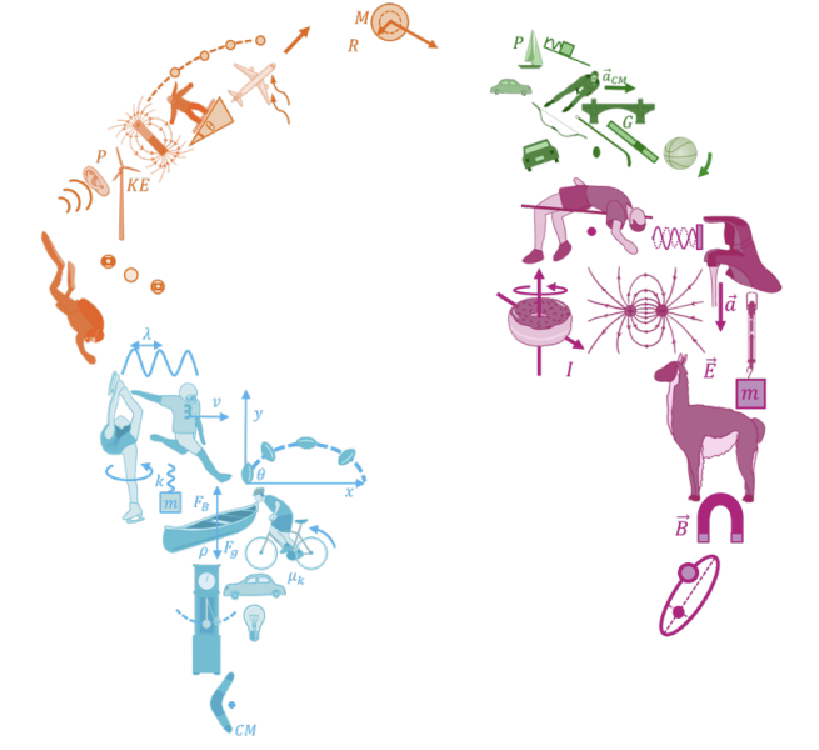
\includegraphics[width=4cm]{figures/BMDW/logo}
\end{textblock*}

\end{frame}

%%%%%%%%%%%%%TOC
\twocolframe{Outline}
  {\tableofcontents[sections={1,2}, subsectionstyle=show/show]\thispagestyle{empty}}
  {\tableofcontents[sections={3}, subsectionstyle=show/show]}
%%%%%%%%%%%%%%%%%%%%%%%%%







%%%%%%%%%%%%%%%%%%%%%%%%%%%%%%%%
\section{The Magnetic Force}
\label{sec:themagneticforce}
\title{The Magnetic Force}


%%%%%%%%%%%%%%%%%%%%%%%%%
\begin{frame}
\titlepage
\thispagestyle{empty}
\end{frame}

%







%%%%%%%%%%%%%%%%%%%%%%%%%%%%%%%
\subsection{Magnetism Basics}
\label{subsec:magnetism}
\twocolframest{Magnetism}
{
\begin{itemize}
\item Some rocks were found to be ``magnetic'' (rather, they were found to attract and repel each other, and they came from a place called Magnesia); ``lodestone''.
\item If you make a needle out of a piece of magnetic material, and suspend it, it kind of points towards the geographic North Pole of the Earth.
\item We call a piece of magnetic material a ``magnet''. We label the side that points towards Earth’s North Pole, the North side of the magnet (cause it points North).
\end{itemize}
}
{
\vspace{-0.5cm}
\capfig{0.75}{figures/Bforce/rock}{https://en.wikipedia.org/wiki/Lodestone}
\vspace{-0.75cm}
\capfig{0.75}{figures/Bforce/compass}{https://www.walmart.ca/en/ip/Pocket-Compass-with-Aluminum-Shell-Edge-for-Outdoor-Camping-Hiking-Sports-Navigation/779N64NE92KJ}
}


%%%%%%%%%%%%%%%%%%%%%%%%%%%%%%

%%%%%%%%%%%%%%%%%%%%%%%%%%%%%%
\begin{bulletframe}{Magnets}
\item With bar magnets, one side (=N) of the magnet always wants to point towards geographic north (ish).
\item We call the other side of the magnet S, since it points to geographic South (ish).
\item It has been observed that the same sides of magnets repel each other (NN or SS), while the opposite sides attract (N-S).
\end{bulletframe}

%%%%%%%%%%%%%%%%%%%%%%%%%%%%%%


%%%%%%%%%%%%%%%%%%%%%%%%%%%%%%
\twocolframesf{Magnetic fields}
{
\vspace{-0.25cm}
\begin{itemize}
\item Fields were introduced as a tool to model ``force at a distance''.
\item Magnetic \textbf{field points in the direction of force on N} (from N to S).
\item Just like electric field lines:
\begin{itemize}
\item Field vector length represented by density of lines.
\item Field vector is tangent to the lines.
\end{itemize}
\item Unlike electric field lines:
\begin{itemize}
\item \textbf{No isolated magnetic charges}, only bar magnets (dipoles).
\item \textbf{Field lines never end}, they are always closed loops.
\end{itemize}
\item The closest analogy with electric charges is that bar magnets are like electric dipoles.
\end{itemize}
}
{
\vspace{-1cm}
\capfig{0.75}{figures/Bforce/edipole}{An electric dipole.}
\vspace{-0.75cm}
\capfig{0.75}{figures/Bforce/barfield}{A magnetic dipole.}
}

%%%%%%%%%%%%%%%%%%%%%%%%%%%%%%




%%%%%%%%%%%%%%%%%%%%%%%%%%%%%%



%%%%%%%%%%%%%%%%%%%%%%%%%%%%%%
\begin{frame}{Cutting up a bar magnet}

\centering
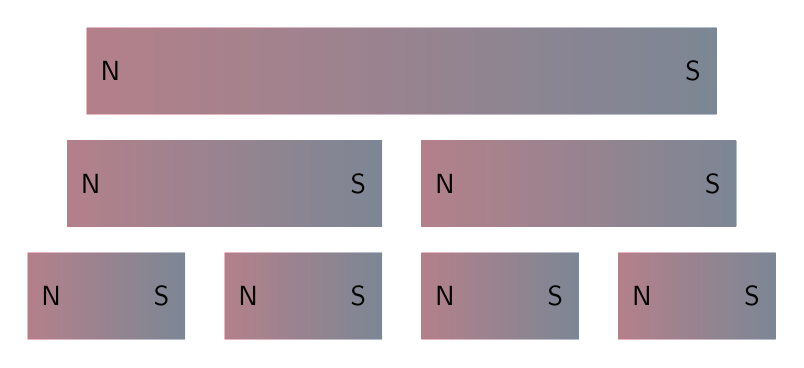
\begin{tikzpicture}{scale=1}
\scalebox{1}
{
\def\L{8}%bar length
\def\h{1.1}%bar height
\def\xs{0.5}%offset
\def\mar{0.3}%margin for N/S label

 \foreach \fac [count=\i] in {1,2,4}
 {
   \def\l{\L/\fac} 
   \def\yb{-\i*\h*1.3}
 
   \foreach \j in {1,...,\fac}{
   \def\xl{-\L/2+(\j-1)*(\l+\xs)-\xs*(\fac-1)/2}
   \fill[left color=qred, right color=qblue, shading=axis,opacity=0.3] ({\xl},\yb-\h/2) rectangle ({\xl+\l}, \yb+\h/2);
   \node at ({\xl+\mar},\yb) {N};
   \node at ({\xl+\l-\mar},\yb) {S};
   }
 }
}
\end{tikzpicture}%
\captionof*{figure}{\textit{When we cut a magnet in 2, we get another magnet (with N and S) sides.}}%
\end{frame}


%%%%%%%%%%%%%%%%%%%%%%%%%%%%%%
\twocolframesf{Tiny bar magnets}
{
\begin{itemize}
\item You can think of magnetic materials as being made up of tiny little bar magnets.
\item The fields for those ``tiny bar magnets'' add up to make the field from a large bar magnet.
\item Those tiny little bar magnets ultimately come from electrons spinning around in atoms:
\begin{itemize}
\item As we will see in next chapter, moving charges create magnetic fields.
\item The electrons spin around the atom.
\item The electrons also spin about their own axis (this is actually the main contribution, and it's Quantum Mechanics).
\end{itemize}
\end{itemize}
}
{
\vspace{-1.2cm}
\capfig{0.75}{figures/Bforce/loopfield}{Magnetic field from a loop of current.}
\vspace{-0.5cm}
\capfig{0.75}{figures/Bforce/barfield}{Magnetic field from a bar magnet.}
}

%%%%%%%%%%%%%%%%%%%%%%%%%%%%%%


%%%%%%%%%%%%%%%%%%%%%%%%%%%%%%
\subsection{Recall: vector-cross product}
\twocolframest{Recall: vector cross-product}
{
\begin{itemize}
\item If we have two vectors, $\vec a$ and $\vec b$, we can define the cross-product:
\begin{align*}%
\vec c = \vec a \times \vec b
\end{align*}%
\begin{itemize}
\item $\vec c$ is perpendicular to both $\vec a$ and $\vec b$.
\item  and has magnitude: $c=ab\sin\theta$
\end{itemize}
\item You can always move vectors around, so easiest to draw them tail to tail before taking cross product
\item Use right hand rule to figure which way $\vec c$ points
\end{itemize}
}
{
\centering
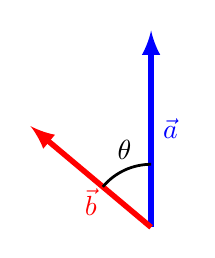
\begin{tikzpicture}{scale=1}
\scalebox{1}
{
\draw[-latex, line width=2,color=blue] (0,0) -- (90:2.5) node[midway,right] {$\vec a$};
\draw[-latex, line width=2,color=red] (0,0) -- (140:2) node[midway,below] {$\vec b$};
\draw[line width = 1.] (90:0.8) arc(90:140:0.8) node[midway,above] {$\theta$};
}
\end{tikzpicture}%
\captionof*{figure}{\textit{Vectors, $\vec a$ and $\vec b$. }}%
}



%%%%%%%%%%%%%%%%%%%%%%%%%%%%%%
\subsection{RIght hand rule(s)}
\twocolframesf{Two right-hand rules}
{
\begin{enumerate}
\item A cross-product between two vectors. Right-hand rule for cross-product.
\begin{align*}%
\vec c = \vec a \times \vec b
\end{align*}%
\vspace{1cm}
\item When you need to relate rotation to a vector. Right-hand rule for axial vectors.
\end{enumerate}
}
{
\vspace{-1cm}
\capfig{0.4}{figures/Bforce/hand}{Right-hand rule for cross-product.}
\vspace{-0.5cm}
\capfig{0.4}{figures/Bforce/axishand}{Right-hand rule for axial vectors.}
}



%%%%%%%%%%%%%%%%%%%%%%%%%%%%%%
\subsection{Force on a moving charge}
\label{subsec:forceonamovingcharge}
\begin{bulletframe}{Force on a moving charge}
\item If a moving charge is in a magnetic field, it experiences a force:
\begin{align*}
\vec F = q \vec v \times \vec B
\end{align*}
\item The magnitude of the force is:
\begin{align*}
F=qvB\sin\theta
\end{align*}
\item[$\rightarrow$] We ultimately use this to define the magnetic field (which is clearly not as pretty as for the electric field). That is, we infer $B$ from the magnitude of the force, $F$.
\end{bulletframe}


%%%%%%%%%%%%%%%%%%%%%%%%%%%%%%


%%%%%%%%%%%%%%%%%%%%%%%%%%%%%%



%%%%%%%%%%%%%%%%%%%%%%%%%%%%%%
\begin{bulletframe}{Work done by a constant magnetic field on a moving charge}
\item The force is always perpendicular to the velocity:
\begin{align*}
\vec F = q \vec v \times \vec B
\end{align*}
\item The displacement is always parallel to the velocity, 
\item The force is thus always perpendicular to the displacement (scalar product is 0)
\item[$\rightarrow$] The magnetic force can do no work; it cannot change the kinetic energy. 
\item[$\rightarrow$] The magnetic force can only change the direction of the velocity, not it’s magnitude.
\end{bulletframe}



%%%%%%%%%%%%%%%%%%%%%%%%%%%%%%




%%%%%%%%%%%%%%%%%%%%%%%%%%%%%%
\subsection{Magnetic force on a charged particle}
\label{subsec:magneticforceonachargedparticle}
\twocolframest{Magnetic force on a charged particle}
{
\begin{align*}
\vec F = q \vec v \times \vec B
\end{align*}
\begin{itemize}
\item Some observations:
\begin{itemize}
\item Always perpendicular to both $\vec v$ and $\vec B$ (cross-product).
\item Can do no work.
\item Proportional to electric charge.
\item No magnetic force on a charge at rest.\only<2>{\textcolor{red}{$\rightarrow$ This should make you uncomfortable, why?}}
\end{itemize}
\end{itemize}
}
{
\only<2>{
\capfig{0.6}{figures/Bforce/einstein}{https://en.wikipedia.org/wiki/Albert\_Einstein\_in\_popular\_culture}
}
}


%%%%%%%%%%%%%%%%%%%%%%%%%%%%%%
\twocolframest{FYI Magnetic force on a charged particle}
{
\begin{itemize}
\only<1>{
\item How does the magnetic force know that humans are predominantly right-handed? For example, how would you explain the right-hand rule to an Alien, who has no concept of right and left?}
\only<2>{
\item Remember: There is no such thing as a force, a magnetic field, an electric field, etc. They are all just mathematical constructs. }
\only<3>{
\item Physical Laws cannot depend on humans being right-handed:	
\begin{itemize}
\item We observe that when an electron is near a source of magnetic field (e.g. a current carrying wire), it moves in a certain direction.
\item We use our right hand to define a thing called the magnetic field.
\item We use our right hand again to determine the force from the magnetic field.
\item[$\rightarrow$] Any physical observation (e.g. which way an electron is deflected) depends on using your right hand twice $\rightarrow$ Then, you could also use your left hand, as once you do two cross products, it doesn't matter which hand you used (don't try this at home, unless you are 100\% sure that you understand the argument!)
\end{itemize}
}
\end{itemize}
}
{
}



%%%%%%%%%%%%%%%%%%%%%%%%%%









\begin{bulletframe}{Force on a moving charge}
\item If a moving charge is in a magnetic field, it experiences a force:
\begin{align*}
\vec F = q \vec v \times \vec B
\end{align*}
\item The magnetic force:
\begin{itemize}
\item Only exerted on a moving charge.
\item Does no work.
\item Perpendicular to magnetic field.
\item Perpendicular to velocity.
\item Magnitude: $qvB\sin\theta$.
\item Direction: RHR.
\end{itemize}
\end{bulletframe}

%%%%%%%%%%%%%%%%%%%%%%%%%%%%%%
\subsection{Right hand rule for vector/cross product}
\label{subsec:righthandruleforvector/cross product}
\twocolframesf{Right hand rule for vector/cross product}
{
The cross-product between two vectors. 
\begin{align*}%
\vec c = \vec a \times \vec b
\end{align*}%
\textbf{Magnitude:} $ab\sin\theta$\\
\textbf{Direction:} Right hand rule. The product is always perpendicular to the plane formed by $\vec a$ and $\vec b$. \\
It does not commute:
\begin{align*}
\vec a \times \vec b = -\vec b \times \vec a
\end{align*}
}
{
\vspace{-1cm}
\capfig{1}{figures/Bforce/hand}{Right-hand rule for cross-product.}

}

%%%%%%%%%%%%%%%%%%%%%%%%%%%%%%



%%%%%%%%%%%%%%%%%%%%%%%%%%%%%%






\section{The Magnetic Field}
\label{sec:themagneticfield}
\title{The Magnetic Field}


%%%%%%%%%%%%%%%%%%%%%%%%%
\begin{frame}
\titlepage
\thispagestyle{empty}
\end{frame}





%%%%%%%%%%%%%%%%%%%%%%%
\subsection{Electron in a magnetic field}
\label{subsec:electroninamagneticfield}
\twocolframesf{Electron in a magnetic field}
{
\begin{itemize}
\item<1-> An electron enters a region of space\only<2->{ with a magnetic field perpendicular to its velocity}
\item<2-> The magnetic force is always perpendicular to the velocity:
\only<3->{
\begin{itemize}
\item Speed is constant (no work).
\item Force is constant in magnitude and perpendicular to velocity.
\item[$\rightarrow$] Uniform circular motion:
\begin{align*}
qvB &= m\frac{v^2}{R}\\
\therefore R &= \frac{m}{q}\frac{v}{B}
\end{align*}
\end{itemize}
}
\end{itemize}
\only<4>{
If the electron has a component of velocity in/out of the page, the path will be a helix.
}
}
{
\centering
\begin{tikzpicture}{scale=1}
\scalebox{1}
{
\def\L{5}
\def\h{5}
\def\Ni{9}
\def\Nj{9}
\def\rad{\L/3}

\only<1>{
\fill[qblue!20] (-1.1*\L/2,-1.1*\h/2) rectangle (1.1*\L/2,1.1*\h/2) node[above=5pt, left,color=qblue!80]{Region of space};
}
\only<2->{
\fill[qblue!20] (-1.1*\L/2,-1.1*\h/2) rectangle (1.1*\L/2,1.1*\h/2) node[above=5pt, left,color=qblue!80]{Region of magnetic field};
\node[left=15pt,below=5pt,color=qblue!80] at (1.1*\L/2,1.1*\h/2) {$\vec B$};
}
\foreach \i in {0,...,\Ni}{
  \def\xi{-\L/2+\i*\L/\Ni}
  \foreach \j in {0,...,\Nj}{
    \def\yj{-\h/2+\j*\h/\Ni}
    \only<2->{
    \node[color=qblue!80, opacity=0.8] at (\xi,\yj) {$\odot$};
    }
  }
}

\only<1>{
\draw[line width = 2, color=qred, -latex]  (1.5*\rad,\rad) -- +(-\rad,0) node[above=7pt, right=16pt] {$\vec v$};
}
\only<1->{
\draw[line width = 2, color=qred, -latex]  (0,\rad) -- +(-\rad,0) node[above=7pt, right=8pt] {$\vec v$};
\fill (0,\rad) circle(2pt);
}
\only<2->{
\draw[line width = 2, color=green!50!black, -latex]  (0,\rad) -- (0,0.3*\rad) node[midway, right] {$\vec F_B$};
}

\only<3->{
\draw[line width = 2] (0,0) circle (\rad);
\draw[line width = 2, color=qred, -latex]  (-\rad,0) -- +(0,-\rad) ;
\draw[line width = 2, color=green!50!black, -latex]   (-\rad,0) -- (-0.3*\rad,0) ;

\draw[line width = 2, color=qred, -latex]  (0,-\rad) -- +(\rad,0) ;
\draw[line width = 2, color=green!50!black, -latex]   (0,-\rad) -- (0,-0.3*\rad) ;

\draw[line width = 2, color=qred, -latex]  (\rad,0) -- +(0,\rad) ;
\draw[line width = 2, color=green!50!black, -latex]   (\rad,0) -- (0.3*\rad,0) ;

\draw[dotted, line width =1.5] (0,0) -- (135:\rad) node[midway, above] {$R$};
}

}
\end{tikzpicture}
}

%%%%%%%%%%%%%%%%%%%%%%%%%%%%%%



%%%%%%%%%%%%%%%%%%%%%%%%%%%%%%
\def\electron at (#1,#2,#3){
\fill[color=myred,opacity=0.8] (#1,#2) circle (#3);
\draw[color=white] (#1-0.8*#3,#2) -- (#1+0.8*#3,#2); %+ sign
\draw[color=white] (#1,#2-0.8*#3) -- (#1,#2+0.8*#3); %+ sign
\draw[color=myred,-latex] (#1,#2+#3) -- (#1,#2+3.5*#3);
}

\def\belectron at (#1,#2,#3){
\fill[color=myred,opacity=0.8] (#1,#2) circle (#3);
\draw[color=white] (#1-0.8*#3,#2) -- (#1+0.8*#3,#2); %+ sign
\draw[color=white] (#1,#2-0.8*#3) -- (#1,#2+0.8*#3); %+ sign
\draw[color=myred,-latex] (#1,#2+#3) -- (#1,#2+3.5*#3);
\draw[color=green!50!black,-latex, line width=1pt] (#1-#3,#2) -- (#1-5*#3,#2);
}

\subsection{Force on a current-carrying wire}
\label{subsec:forceonacurrentcarryingwire}
\twocolframesf{Force on a current-carrying wire}
{
\vspace{-0.25cm}
\begin{itemize}
\item<1-> Current: positive charges moving with a drift velocity, $\vec v_d$. 
\item<2-> One positive charge $e$ feels a force: $\vec F_e = e \vec v_d \times \vec B$
\item<3-> In a segment of length $l$, and area $A$, if there are $n$ charges per unit volume, there are a total of $N$ charges:
$N=nAl$
\item<4-> The total force on those charges is: $\vec F=N\vec F_e=nAle \vec v_d \times \vec B$
\item<5->  Recall, microscopic model of current, $I=nAev_d$
\item<6->  Make  the vector, $\vec l$, in the same direction as, $\vec v_d$: 
\begin{align*}
\boxed{
\vec F = I \vec l \times \vec B}
\end{align*}
\end{itemize}
}
{
\vspace{-1cm}
\centering
\begin{tikzpicture}[scale=0.5,yshift=-6cm]
\scalebox{1}{
  \def\L{7.0}
  \def\R{2}
  \def\er{0.15}
  \def\Ni{7}
  \def\Nj{8}
  
\only<1>{  %empty, just so it doesn't move the figure around
  \fill[qblue!20, opacity=0] (-3*\R,-0.2*\L) rectangle (3*\R,1.2*\L) node[above=5pt, left, color=qblue!80]{Region of magnetic field};
}

\only<2->{  
\fill[qblue!20] (-3*\R,-0.2*\L) rectangle (3*\R,1.2*\L) node[above=5pt, left, color=qblue!80]{Region of magnetic field};
\node[left=7pt,below=2pt,color=qblue!80] at (3*\R,1.2*\L) {$\vec B$};
\foreach \i in {0,...,\Ni}{
  \def\xi{-2.5*\R+.25*\R/\Ni+\i*5*\R/\Ni}
  \foreach \j in {0,...,\Nj}{
    \def\yj{\j*\L/\Ni-\L/\Nj/2}
    \node[color=qblue!80, opacity=0.8] at (\xi,\yj) {$\times$};
  }
}

}
\only<1>{
  \foreach \i in {0,...,3}{
    \def\yj{0.25*\L+\i*\L/8}
    \electron at (0,\yj,\er);
    \electron at (-\R/2,\yj,\er);
    \electron at (\R/2,\yj,\er);
    
    \electron at (-0.75*\R,\yj+\L/16,0.9*\er);
    \electron at (-0.25*\R,\yj+\L/16,0.9*\er);
    \electron at (0.25*\R,\yj+\L/16,0.9*\er);
    \electron at (0.75*\R,\yj+\L/16,0.9*\er);
  }
  }
  
  \only<2->{
  \foreach \i in {0,...,3}{
    \def\yj{0.25*\L+\i*\L/8}
    \belectron at (0,\yj,\er);
    \belectron at (-\R/2,\yj,\er);
    \belectron at (\R/2,\yj,\er);
    
    \belectron at (-0.75*\R,\yj+\L/16,0.9*\er);
    \belectron at (-0.25*\R,\yj+\L/16,0.9*\er);
    \belectron at (0.25*\R,\yj+\L/16,0.9*\er);
    \belectron at (0.75*\R,\yj+\L/16,0.9*\er);
  }
  
  }
  
%cylinder:
  \fill[top color=gray!15!black,bottom color=gray!20,shading=axis,opacity=0.3, draw=black] (-\R,0) arc (180:360:{\R} and {\R/4}) --  (\R,\L) arc (360:180:{\R} and {\R/4}) -- (-\R,0); 
  \draw[dashed] (\R,0) arc (0:180:{\R} and {\R/4}) ;
  \fill[color=gray!90,opacity=0.5,draw=black] (\R,\L) arc (0:360:{\R} and {\R/4});
%%%%%%  
  \fill[top color=myred!30,bottom color=myred!80,shading=axis,opacity=0.3, draw=black] (-\R,0.25*\L) arc (180:360:{\R} and {\R/4}) --  (\R,0.75*\L) arc (360:180:{\R} and {\R/4}) -- (-\R,0.25*\L); 
  \draw[dashed,color=myred!30] (\R,0.25*\L) arc (0:180:{\R} and {\R/4}) ;
  \fill[color=myred!90,opacity=0.3,draw=myred] (\R,0.75*\L) arc (0:360:{\R} and {\R/4});   
  
  %

  \draw[line width=2pt,-latex] (-1.3*\R,0.4*\L) -- (-1.3*\R,0.6*\L) node[midway,left]{$\vec v_d$};
  \draw[line width=2pt,-latex,color=myred] (1.3*\R,0.35*\L) -- (1.3*\R,0.65*\L) node[midway,right]{$I$};
  \only<2->{
  %\node[color=green!50!black] at (0,0.15*\L) {\Large $\vec F_e$};
  \node[color=green!50!black] at (-1.4*\R,0.85*\L) {\Large $\vec F_e$};
  }
  
  \only<3-5>{
    \draw[line width=1pt,latex-latex] (-1.9*\R,0.25*\L) -- (-1.9*\R,0.75*\L) node[midway,left]{$l$};
    \node at (0,\L) {$A$};
  }
  
  \only<6>{
    \draw[line width=1pt,line width=2pt,-latex] (-1.9*\R,0.25*\L) -- (-1.9*\R,0.75*\L) node[midway,left=3pt]{\Large $\vec l$};
    \node at (0,\L) {$A$};
  }
}
\end{tikzpicture}
\captionof*{figure}{\textit{Positive charges drifting with an average velocity, $\vec v_d$. Would you come to different conclusions modelling electrons drifting downwards?}}
}



%%%%%%%%%%%%%%%%%%%%%%%%%%%%%%
\twocolframesf{Force on a current-carrying wire (in general)}
{
\begin{itemize}
\item On a section of length, $dl$ :
\begin{align*}
d\vec F = I d\vec l \times \vec B
\end{align*}
\item On a wire made of many sections:
\begin{align*}
\vec F = \int d\vec F = I \int d \vec l \times \vec B
\end{align*}
\item If it’s just a straight wire of length, $l$,  and the field is uniform
\begin{align*}
\vec F = I \int d \vec l \times \vec B =I \vec l \times \vec B
\end{align*}
\end{itemize}
}
{
\centering
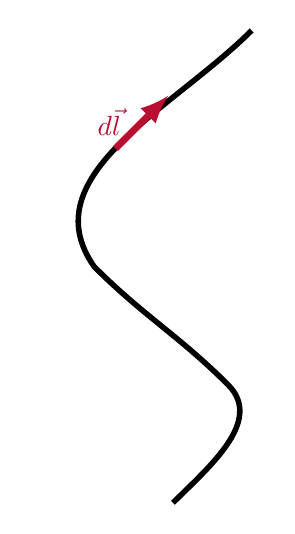
\begin{tikzpicture}[scale=1]
\scalebox{1.0}{
  \draw[line width=2pt] (0,0) to [out=45, in=-45] (0.7,1.5) to [out=135, in=-45] (-1,3) to[out=125,in=225] (1,6);
  \draw[-latex, color=qred, line width =2.5pt] (-0.73,4.5) -- +(45:0.95) node[midway, left=3pt] {$d\vec l$};

}
\end{tikzpicture}
\captionof*{figure}{\textit{The vector $d\vec l$ points in the same direction as the current.}}
}


%%%%%%%%%%%%%%%%%%%%%%%%%%%%%%









%%%%%%%%%%%%%%%%%%%%%%%%%%%%


\def\belectron at (#1,#2,#3){
\fill[color=myred,opacity=0.8] (#1,#2) circle (#3);
\draw[color=white] (#1-0.8*#3,#2) -- (#1+0.8*#3,#2); %+ sign
\draw[color=white] (#1,#2-0.8*#3) -- (#1,#2+0.8*#3); %+ sign
\draw[color=myred,-latex] (#1,#2+#3) -- (#1,#2+3.5*#3);
\draw[color=green!50!black,-latex, line width=1pt] (#1-#3,#2) -- (#1-5*#3,#2);
}


\subsection{Example: force from a wire}
\label{subsec:exampleforcefromawire}
\twocolframesf{Wire of length, $l$, carrying current, $I$, in a magnetic field, $\vec B$.}
{
\vspace{-0.25cm}
\begin{itemize}
\item Current: positive charges moving with a drift velocity, $\vec v_d$. 
\item One positive charge $e$ feels a force: $\vec F_e = e \vec v_d \times \vec B$
\item In a segment of length $l$, and area $A$, if there are $n$ charges per unit volume, there are a total of $N$ charges:
$N=nAl$
\item The total force on those charges is: $\vec F=N\vec F_e=nAle \vec v_d \times \vec B$
\item  Recall, microscopic model of current, $I=nAev_d$
\item  Make  the vector, $\vec l$, in the same direction as, $\vec v_d$: 
\begin{align*}
\boxed{
\vec F = I \vec l \times \vec B}
\end{align*}
\end{itemize}
}
{
%\vspace{-1cm}
\centering
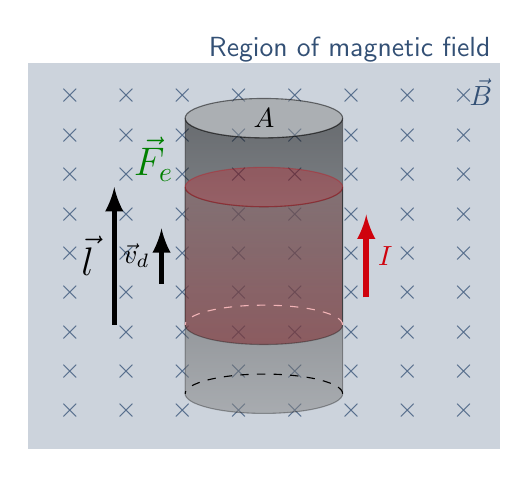
\begin{tikzpicture}[scale=0.5,yshift=-6cm]
\scalebox{1}{
  \def\L{7.0}
  \def\R{2}
  \def\er{0.15}
  \def\Ni{7}
  \def\Nj{8}
  
  \fill[qblue!20] (-3*\R,-0.2*\L) rectangle (3*\R,1.2*\L) node[above=5pt, left, color=qblue!80]{Region of magnetic field};
  \node[left=7pt,below=2pt,color=qblue!80] at (3*\R,1.2*\L) {$\vec B$};
  \foreach \i in {0,...,\Ni}{
    \def\xi{-2.5*\R+.25*\R/\Ni+\i*5*\R/\Ni}
      \foreach \j in {0,...,\Nj}{
        \def\yj{\j*\L/\Ni-\L/\Nj/2}
        \node[color=qblue!80, opacity=0.8] at (\xi,\yj) {$\times$};
       }
   }
 
  \foreach \i in {0,...,3}{
    \def\yj{0.25*\L+\i*\L/8}
    \belectron at (0,\yj,\er);
    \belectron at (-\R/2,\yj,\er);
    \belectron at (\R/2,\yj,\er);
    
    \belectron at (-0.75*\R,\yj+\L/16,0.9*\er);
    \belectron at (-0.25*\R,\yj+\L/16,0.9*\er);
    \belectron at (0.25*\R,\yj+\L/16,0.9*\er);
    \belectron at (0.75*\R,\yj+\L/16,0.9*\er);
  }
  
    
%cylinder:
  \fill[top color=gray!15!black,bottom color=gray!20,shading=axis,opacity=0.3, draw=black] (-\R,0) arc (180:360:{\R} and {\R/4}) --  (\R,\L) arc (360:180:{\R} and {\R/4}) -- (-\R,0); 
  \draw[dashed] (\R,0) arc (0:180:{\R} and {\R/4}) ;
  \fill[color=gray!90,opacity=0.5,draw=black] (\R,\L) arc (0:360:{\R} and {\R/4});
%%%%%%  
  \fill[top color=myred!30,bottom color=myred!80,shading=axis,opacity=0.3, draw=black] (-\R,0.25*\L) arc (180:360:{\R} and {\R/4}) --  (\R,0.75*\L) arc (360:180:{\R} and {\R/4}) -- (-\R,0.25*\L); 
  \draw[dashed,color=myred!30] (\R,0.25*\L) arc (0:180:{\R} and {\R/4}) ;
  \fill[color=myred!90,opacity=0.3,draw=myred] (\R,0.75*\L) arc (0:360:{\R} and {\R/4});   
  
  %

  \draw[line width=2pt,-latex] (-1.3*\R,0.4*\L) -- (-1.3*\R,0.6*\L) node[midway,left]{$\vec v_d$};
  \draw[line width=2pt,-latex,color=myred] (1.3*\R,0.35*\L) -- (1.3*\R,0.65*\L) node[midway,right]{$I$};

  \node[color=green!50!black] at (-1.4*\R,0.85*\L) {\Large $\vec F_e$};

  

    \draw[line width=1pt,line width=2pt,-latex] (-1.9*\R,0.25*\L) -- (-1.9*\R,0.75*\L) node[midway,left=3pt]{\Large $\vec l$};
    \node at (0,\L) {$A$};

}
\end{tikzpicture}
\captionof*{figure}{\textit{Positive charges drifting with an average velocity, $\vec v_d$. Would you come to different conclusions modelling electrons drifting downwards?}}
}



%%%%%%%%%%%%%%%%%%%%%%%%
\twocolframesf{Force on a current-carrying wire (in general)}
{
\begin{itemize}
\item On a section of length, $dl$ :
\begin{align*}
d\vec F = I d\vec l \times \vec B
\end{align*}
\item On a wire made of many sections:
\begin{align*}
\vec F = \int d\vec F = I \int d \vec l \times \vec B
\end{align*}
\item If it’s just a straight wire of length, $l$,  and the field is uniform
\begin{align*}
\vec F = I \int d \vec l \times \vec B =I \vec l \times \vec B
\end{align*}
\end{itemize}
}
{
\centering
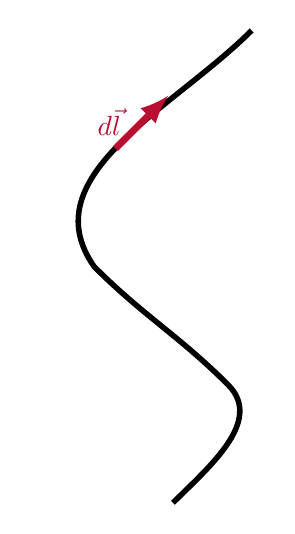
\begin{tikzpicture}[scale=1]
\scalebox{1.0}{
  \draw[line width=2pt] (0,0) to [out=45, in=-45] (0.7,1.5) to [out=135, in=-45] (-1,3) to[out=125,in=225] (1,6);
  \draw[-latex, color=qred, line width =2.5pt] (-0.73,4.5) -- +(45:0.95) node[midway, left=3pt] {$d\vec l$};

}
\end{tikzpicture}
\captionof*{figure}{\textit{The vector $d\vec l$ points in the same direction as the current.}}
}


%%%%%%%%%%%%%%%%%%%%%%%%%%%



\section{The Magnetic Torque}
\label{sec:themagnetictorque}
\title{The Magnetic Torque}


%%%%%%%%%%%%%%%%%%%%%%%%%
\begin{frame}
\titlepage
\thispagestyle{empty}
\end{frame}



%%%%%%%%%%%%%%%%%%%%%%%%
\subsection{Torque on a current-carrying loop}
\label{subsec:torqueonacurrentcarryingloop}
\twocolframest{Torque on a current-carrying loop}
{
\begin{itemize}
\item The force on either segment:\\ $F=ILB$
\item The torque from one segment:\\ $\tau_s = \left(\frac{d}{2}\right)F=\frac{d}{2}ILB$
\item The total torque (when there is no magnetic flux through the loop):\\ $\tau = 2\tau_s=IdLB=\textcolor{red}{IA}B=\textcolor{red}{\mu}B$
\item We introduce the \textbf{magnetic moment}, $\mu$, of a current carrying loop of area $A$:
\begin{align*}
\mu &= IA\\
\therefore \tau &= \mu B
\end{align*}
\end{itemize}
The torque must depend on the orientation of the loop...
}
{
\centering
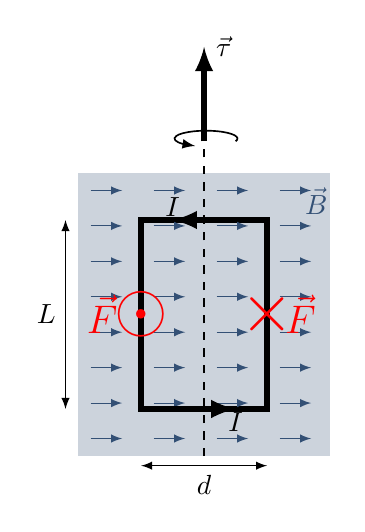
\begin{tikzpicture}[scale=0.4]
\scalebox{1}{
\def\L{4}
\def\h{6}
\def\N{8}

\fill[qblue!20] (-\L,-1.5*\h/2) rectangle (\L,1.5*\h/2) ;%node[above=10pt, left, color=qblue!80]{Region of magnetic field};
\draw[line width=2] (-\L/2,-\h/2) rectangle (\L/2,\h/2);



\foreach \i in {0,...,7}{
 \def\yi{-1.5*\h/2+\i*1.5*\h/\N+1.5*\h/\N/2}
 
 \draw[-latex, color=qblue!80](-0.9*\L,\yi) -- +(1,0);
 \draw[-latex, color=qblue!80](-0.4*\L,\yi) -- +(1,0);
 \draw[-latex, color=qblue!80](0.1*\L,\yi) -- +(1,0);
 \draw[-latex, color=qblue!80](0.6*\L,\yi) -- +(1,0);

}

\node[left=5pt, below=2pt,color=qblue!80] at (\L,1.5*\h/2) {$\vec B$};
\draw[-latex, color=black, line width =2pt] (-0.25*\L,-\h/2) -- (0.25*\L,-\h/2) node[below=-3pt] {$I$};
\draw[latex-, color=black, line width =2pt]  (-0.25*\L,\h/2) node[above=-3pt] {$I$} -- (0.25*\L,\h/2);
\draw[latex-latex] (-\L/2,-1.6*\h/2) -- (\L/2,-1.6*\h/2) node[midway, below] {$d$};
\draw[latex-latex] (-1.1*\L,-\h/2) -- (-1.1*\L,\h/2) node[midway, left] {$L$};

%axis of rotation
\draw[dashed, line width = 1pt] (0,-1.5*\h/2) -- (0,1.5*\h/2+1);
\draw[-latex, color=black, line width =2pt] (0,1.5*\h/2+1) -- +(0,3) node[right]{$\vec\tau$};
\draw[-latex,line width = 0.6pt] (1,1.5*\h/2+1) arc(-20:250:1 and 0.25);

\node[color=red] at (-\L/2,0) {\Huge $\odot$};
\node[color=red,left=5pt] at (-\L/2,0) {\Large $\vec F$ };
\node[color=red] at (\L/2,0) {\Huge $\times$};
\node[color=red,right=3pt] at (\L/2,0) {\Large $\vec F$ };
}
\end{tikzpicture}
\captionof*{figure}{\textit{A rectangular loop carrying counter-clockwise current, $I$.}}
} 


%%%%%%%%%%%%%%%%%%%%%%%%
\subsection{Magnetic moment}
\twocolframesf{Magnetic moment}
{
\begin{itemize}
\item Define the magnetic moment, $\vec \mu$, for a loop of area $A$ carrying current $I$:
\begin{align*}
\vec \mu = I \vec A
\end{align*}
\item Direction of $\vec A$, $\vec \mu$, given by normal to the surface, direction of current, and right hand rule for axial vectors.
\item Torque on a loop given by:
\begin{align*}
\vec \tau = \vec \mu \times \vec B
\end{align*}
\item This is analogous to the torque on an electric dipole from an electric field (electric dipole moment $\vec p \rightarrow \vec \mu$ magnetic moment)
\end{itemize}
}
{
\capfig{0.8}{figures/Bforce/momenthand}{Using the right-hand rule for axial current to determine the direction of the magnetic moment of a loop carrying current, $I$.}
The net torque on the loop always acts to make $\vec\mu$ and $\vec B$ parallel.

}

%%%%%%%%%%%%%%%%%%%%%%%%


%%%%%%%%%%%%%%%%%%%%%%%%


%%%%%%%%%%%%%%%%%%%%%%%%
\def\electron at (#1,#2,#3){
\fill[color=myred,opacity=0.8] (#1,#2) circle (#3);
\draw[color=white] (#1-0.8*#3,#2) -- (#1+0.8*#3,#2);%- sign
} 

\def\velectron at (#1,#2,#3){
\fill[color=myred,opacity=0.8] (#1,#2) circle (#3);
\draw[color=white] (#1-0.8*#3,#2) -- (#1+0.8*#3,#2);%- sign
\draw[-latex] (#1+#3,#2) -- (#1+5*#3,#2);%speed
} 

\def\fvelectron at (#1,#2,#3){
\fill[color=myred,opacity=0.8] (#1,#2) circle (#3);
\draw[color=white] (#1-0.8*#3,#2) -- (#1+0.8*#3,#2);%- sign
\draw[-latex] (#1+#3,#2) -- (#1+5*#3,#2);%speed
\draw[color=green!70!black,-latex, line width=0.4pt] (#1,#2-#3) -- (#1,#2-5*#3);%force
}
\def\ffvelectron at (#1,#2,#3){
\fill[color=myred,opacity=0.8] (#1,#2) circle (#3);
\draw[color=white] (#1-0.8*#3,#2) -- (#1+0.8*#3,#2);%- sign
\draw[-latex] (#1+#3,#2) -- (#1+5*#3,#2);%speed
\draw[color=green!50!black,-latex, line width=0.4pt] (#1,#2-#3) -- (#1,#2-5*#3);%force
\draw[color=qred,-latex, line width=0.4pt] (#1,#2+#3) -- (#1,#2+5*#3);%force
}



\subsection{The Hall effect}
\label{subsec:thehalleffect}
\twocolframe{The Hall Effect}
{
\only<1-5>{
\begin{itemize}
\item<1-> We have a strip of metal immersed in a magnetic field into the page, as shown.
\begin{enumerate}
\item<1-> The electrons are at rest in the metal that is immersed in the magnetic field.
\item<2-> Apply a potential difference to the metal, electrons start moving.
\item<3-> Electrons are deflected downwards because of the magnetic field.
\item<4-> The bottom of the strip becomes more negative resulting in an \textbf{electric force} opposite of the magnetic force. 
\item<5-> This leads to the Hall voltage, $\Delta V_H$.
\end{enumerate}
\end{itemize}
}
\only<6>{
\textbf{By measuring the Hall voltage, you can measure $B$. A Hall probe!}
\begin{align*}
\textcolor{qred}{\vec F_E}+\textcolor{green!70!black}{\vec F_B}&=0\\
\therefore qE&=qvB\\
\frac{\Delta V_H}{d}&=vB=\frac{I}{neA}B\\
\therefore \Delta V_H&=\frac{Id}{neA}B
\end{align*}
where $v$ is the drift velocity and we made use of our model for current.
}
}
{%
\only<4>{
\begin{align*}
\textcolor{qred}{\vec F_E}+\textcolor{green!70!black}{\vec F_B}=0
\end{align*}
}


%\vspace{-1cm}%
\centering %
\begin{tikzpicture}[scale=1]%
  \def\h{2.0}%
  \def\L{5.0}%
  \def\er{0.07}%
  \def\Ni{7}%
  \def\Nj{5}%
%  
% 
  \fill[qblue!20] (-0.6*\L,-0.6*\h) rectangle (0.6*\L,0.6*\h) ;%node[above=5pt, left, color=qblue!80]{Region of magnetic field};
  \node[left=7pt,below=2pt,color=qblue!80] at (0.6*\L,0.6*\h) {$\vec B$};
  \foreach \i in {0,...,\Ni}{
    \def\xi{-0.55*\L+.25*\L/\Ni+\i*\L/\Ni}
      \foreach \j in {0,...,\Nj}{
        \def\yj{-0.5*\h+\j*\h/\Nj}
        \node[color=qblue!80, opacity=0.8] at (\xi,\yj) {$\times$};
       }
   }
%  
  %piece of metal
  \fill[black!60,opacity=0.7] (-0.4*\L,-0.25*\h) rectangle (0.4*\L,0.25*\h);
%  
  %circuit to drive electrons
  \only<2->{
  \draw[line width =1.5pt] (-0.4*\L,0) -- (-0.5*\L,0) -- (-0.5*\L,-\h) -- (-0.02*\L,-\h);
  \draw[line width =1.5pt] (0.4*\L,0) -- (0.5*\L,0) -- (0.5*\L,-\h) -- (0.02*\L,-\h);
  \draw[line width =1.5pt] (-0.02*\L,-\h-0.1*\h) -- (-0.02*\L,-\h+0.1*\h) node[left]{\small $-$};
  \draw[line width =1.5pt] (0.02*\L,-\h-0.2*\h) -- (0.02*\L,-\h+0.2*\h) node[right] {\small $+$};
  }%
%
  %electrons alone
  \only<1>{
  \foreach \ie in {0,...,6}{
    \def\xi{-0.3*\L+\ie*0.6*\L/6}
    \electron at (\xi,0,\er);
    \electron at (\xi-0.05*\L,0.2*\h,\er);
    \electron at (\xi-0.05*\L,-0.2*\h,\er);
  } %plus 2 at the end to look prettier
  \electron at (0.4*\L-0.05*\L,0.2*\h,\er);
  \electron at (0.4*\L-0.05*\L,-0.2*\h,\er);
  }
%   
  %electrons with v
  \only<2>{
  \foreach \ie in {0,...,6}{
    \def\xi{-0.3*\L+\ie*0.6*\L/6}
    \velectron at (\xi,0,\er);
    \velectron at (\xi-0.05*\L,0.2*\h,\er);
    \velectron at (\xi-0.05*\L,-0.2*\h,\er);
  } %plus 2 at the end to look prettier
  \velectron at (0.4*\L-0.05*\L,0.2*\h,\er);
  \velectron at (0.4*\L-0.05*\L,-0.2*\h,\er);
  }
%  
  %electrons with v and F
  \only<3>{
  \foreach \ie in {0,...,6}{
    \def\xi{-0.3*\L+\ie*0.6*\L/6}
    \fvelectron at (\xi,0,\er);
    \fvelectron at (\xi-0.05*\L,0.2*\h,\er);
    \fvelectron at (\xi-0.05*\L,-0.2*\h,\er);
  } %plus 2 at the end to look prettier
  \fvelectron at (0.4*\L-0.05*\L,0.2*\h,\er);
  \fvelectron at (0.4*\L-0.05*\L,-0.2*\h,\er);
  }
% 
  %electrons with v
  \only<4>{
  \foreach \ie in {0,...,6}{
    \def\xi{-0.3*\L+\ie*0.6*\L/6}
    \ffvelectron at (\xi,-0.1*\h,\er);
    \ffvelectron at (\xi-0.05*\L,0,\er);
    \ffvelectron at (\xi-0.05*\L,-0.2*\h,\er);
  } %plus 2 at the end to look prettier
  \ffvelectron at (0.4*\L-0.05*\L,0,\er);
  \ffvelectron at (0.4*\L-0.05*\L,-0.2*\h,\er);
  }
%  
  \only<5->{
  %voltage
   \draw[latex-latex, line width=2, color=qred] (0,-0.25*\h) -- (0,0.25*\h) node[midway,left] {$\Delta V_H$} node[midway,right] {$d$};
   \node[below,color=qred] at (0,-0.25*\h) {$-$};
   \node[above,color=qred] at (0,0.25*\h) {$+$};
   %conventional current
   \draw[-latex, line width =1.5pt] (0.2*\L,-\h) -- (0.4*\L,-\h) node[midway, below] {$I$};
  }
%  
\end{tikzpicture}
\captionof*{figure}{\textit{\only<1->{A piece of conducting material in a magnetic field.}\only<2->{ A current is driven by a potential difference}\only<3->{ Negative charges are deflected downwards.}\only<4->{ This causes a buildup of negative charge on the bottom} \only<5->{, leading a potential difference between the top and bottom, the ``Hall Voltage''.}}}
}


%%%%%%%%%%%%%%%%%%%%%%%%
\def\vpositron at (#1,#2,#3){
\fill[color=myred,opacity=0.8] (#1,#2) circle (#3);
\draw[color=white] (#1-0.8*#3,#2) -- (#1+0.8*#3,#2);%- sign
\draw[color=white] (#1,#2-0.8*#3) -- (#1,#2+0.8*#3);%- sign
\draw[-latex] (#1-#3,#2) -- (#1-5*#3,#2);%speed
} 

\def\fvpositron at (#1,#2,#3){
\fill[color=myred,opacity=0.8] (#1,#2) circle (#3);
\draw[color=white] (#1-0.8*#3,#2) -- (#1+0.8*#3,#2);%- sign
\draw[color=white] (#1,#2-0.8*#3) -- (#1,#2+0.8*#3);%- sign
\draw[-latex] (#1-#3,#2) -- (#1-5*#3,#2);%speed
\draw[color=green!70!black,-latex, line width=0.4pt] (#1,#2-#3) -- (#1,#2-5*#3);%force
} 


\subsection{The sign of charge carriers}
\label{subsec:thesignofchargecarriers}
\twocolframe{The sign of charge carriers}
{
Can we tell if current is carried by positive or negative charges?
\begin{itemize}
\item<1-> What happens if it's actually positive charges carrying current? Their speed is in the opposite direction.
\item<2-> The magnetic force is downwards, leading to a net positive charge at the bottom of the strip. 
\item<3-> The Hall voltage is now the opposite sign! By measuring the Hall voltage, you can determine that it is negative charges that are actually moving!
\end{itemize}

}
{%
\centering %
\begin{tikzpicture}[scale=1]%
  \def\h{2.0}%
  \def\L{5.0}%
  \def\er{0.07}%
  \def\Ni{7}%
  \def\Nj{5}%
%  
% 
  \fill[qblue!20] (-0.6*\L,-0.6*\h) rectangle (0.6*\L,0.6*\h) ;%node[above=5pt, left, color=qblue!80]{Region of magnetic field};
  \node[left=7pt,below=2pt,color=qblue!80] at (0.6*\L,0.6*\h) {$\vec B$};
  \foreach \i in {0,...,\Ni}{
    \def\xi{-0.55*\L+.25*\L/\Ni+\i*\L/\Ni}
      \foreach \j in {0,...,\Nj}{
        \def\yj{-0.5*\h+\j*\h/\Nj}
        \node[color=qblue!80, opacity=0.8] at (\xi,\yj) {$\times$};
       }
   }
%  
  %piece of metal
  \fill[black!60,opacity=0.7] (-0.4*\L,-0.25*\h) rectangle (0.4*\L,0.25*\h);
%  
  %circuit to drive electrons
  \draw[line width =1.5pt] (-0.4*\L,0) -- (-0.5*\L,0) -- (-0.5*\L,-\h) -- (-0.02*\L,-\h);
  \draw[line width =1.5pt] (0.4*\L,0) -- (0.5*\L,0) -- (0.5*\L,-\h) -- (0.02*\L,-\h);
  \draw[line width =1.5pt] (-0.02*\L,-\h-0.1*\h) -- (-0.02*\L,-\h+0.1*\h) node[left]{\small $-$};
  \draw[line width =1.5pt] (0.02*\L,-\h-0.2*\h) -- (0.02*\L,-\h+0.2*\h) node[right] {\small $+$};

%
  %electrons with v
  \only<1>{
  \foreach \ie in {0,...,6}{
    \def\xi{-0.3*\L+\ie*0.6*\L/6}
    \vpositron at (\xi,0,\er);
    \vpositron at (\xi-0.05*\L,0.2*\h,\er);
    \vpositron at (\xi-0.05*\L,-0.2*\h,\er);
  } %plus 2 at the end to look prettier
  \vpositron at (0.4*\L-0.05*\L,0.2*\h,\er);
  \vpositron at (0.4*\L-0.05*\L,-0.2*\h,\er);
  }
  
  %electrons with v and f
  \only<2>{
  \foreach \ie in {0,...,6}{
    \def\xi{-0.3*\L+\ie*0.6*\L/6}
    \fvpositron at (\xi,0,\er);
    \fvpositron at (\xi-0.05*\L,0.2*\h,\er);
    \fvpositron at (\xi-0.05*\L,-0.2*\h,\er);
  } %plus 2 at the end to look prettier
  \fvpositron at (0.4*\L-0.05*\L,0.2*\h,\er);
  \fvpositron at (0.4*\L-0.05*\L,-0.2*\h,\er);
  }  
  \only<3->{
  %voltage
   \draw[latex-latex, line width=2, color=qred] (0,-0.25*\h) -- (0,0.25*\h) node[midway,left] {$\Delta V_H$} node[midway,right] {$d$};
   \node[below,color=qred] at (0,-0.25*\h) {$+$};
   \node[above,color=qred] at (0,0.25*\h) {$-$};
  }
   %conventional current
   \draw[-latex, line width =1.5pt] (0.2*\L,-\h) -- (0.4*\L,-\h) node[midway, below] {$I$};
  
%  
\end{tikzpicture}
}

%%%%%%%%%%%%%%%%%%%%%%%%




%%%%%%%%%%%%%%%%%%%%%%%%
\subsection{The Lorentz force and velocity selector}
\label{subsec:thelorentzforceandvelocityselector}
\twocolframesf{The Lorentz force and velocity selector}
{%
\begin{itemize}
\item If a charge is placed in both magnetic and electric fields, it will feel a force (the Lorentz Force):%
\begin{align*}
\vec F = q\vec E+q\vec v \times \vec B
\end{align*}
\item We can build a ``velocity selector'' by having perpendicular electric and magnetic fields.%
\item Only particles with the ``selected velocity'' make it through without hitting the plates:%
\begin{align*}
qE & = qvB\\
\therefore v&=\frac{E}{B}
\end{align*}
\end{itemize}
}
{
\centering %
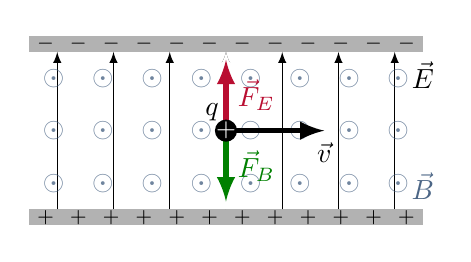
\begin{tikzpicture}[scale=1]%
  \def\h{2.0}%
  \def\L{5.0}%
  \def\d{0.2}
  \def\w{2}
  \def\Ni{12}
  \def\Nie{7}
  \def\Nib{8}
  
  %charged plates:
  \fill[color = black!30] (-\L/2, \h/2) rectangle (\L/2, \h/2+\d);
  \fill[color = black!30] (-\L/2, -\h/2) rectangle (\L/2, -\h/2-\d);  
  \foreach \i in {1,...,\Ni}{
    \def\xi{-\L/2+\i*\L/\Ni-\L/2/\Ni} 
    \node at (\xi, \h/2+\d/2) {\scriptsize $-$};
    \node at (\xi, -\h/2-\d/2) {\scriptsize $+$};
  }
  %Efield lines
    \foreach \i in {1,...,\Nie}{
    \def\xi{-\L/2+\i*\L/\Nie-\L/2/\Nie} 
    \draw [-latex] (\xi,-\h/2) -- (\xi,\h/2) ;
  }
  \draw [color=white,-latex] (0,-\h/2) -- (0,\h/2) ;
  %Bfield
  \foreach \i in {1,...,\Nib}{
    \def\xi{-\L/2+\i*\L/\Nib-\L/2/\Nib} 
      \foreach \j in {1,...,3}{
        \def\yj{-0.5*\h+\j*\h/3-\h/6.0}
        \node[color=qblue!70, opacity=0.8] at (\xi,\yj) {$\odot$};
       }
   }
   
   %particle
   
   \draw[-latex, line width = 2] (0,0) -- +(\L/4,0) node[below] {$\vec v$};
   \draw[-latex, line width = 2, color=qred] (0,0) -- +(0,0.45*\h) node[midway,right] {$\vec F_E$};
   \draw[-latex, line width = 2, color=green!50!black] (0,0) -- +(0,-0.45*\h) node[midway,right] {$\vec F_B$};
   \fill[color=black] (0,0) circle (4pt);
   
   \node[left=5pt,above] at (0,0) {$q$};
   \node[color=white] at (0,0) {\small $+$};
   \node[left, above,color=qblue!70] at (\L/2,-\h/2) {$\vec B$};
   \node[left, below] at (\L/2,\h/2) {$\vec E$};
   
\end{tikzpicture}
\captionof*{figure}{\textit{A velocity selector is designed with perpendicular electric and magnetic fields. The resulting forces cancel if $q$ has the right velocity.}}
}




%%%%%%%%%%%%%%%%%%%%%%%%
\subsection{The mass spectrometer}
\label{subsec:themassspectrometer}
\twocolframe{The mass spectrometer}
{%
\begin{itemize}
\item Material is vaporized, ionizing to be accelerated towards the velocity selector. Only those with speed, $v$, enter the mass spectrometer:
\begin{align*}
qvB &= m\frac{v^2}{r}\\
\therefore \frac{m}{q} &= \frac{rB}{v} =\frac{rBB'}{E'}
\end{align*}
\item Since $q=\pm ne$ for ions, one can determine the mass of the ions in the sample, hence the name.
\end{itemize}
}
{
\vspace{-0.5cm}
\centering %
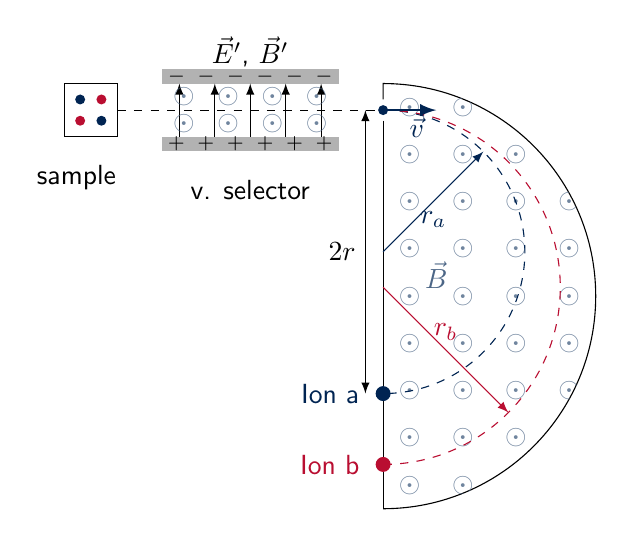
\begin{tikzpicture}[scale=0.9]%

\def\R{3}
\def\ra{2}
\def\rb{2.5}
\def\ya{7/8*\R-2*\ra}
\def\yb{7/8*\R-2*\rb}
\def\Lv{2.5} %length of v selector

%sample 
\draw (-1.5*\Lv-0.25*\R,0.75*\R) rectangle (-1.5*\Lv,\R);
\fill[color=qred] (-1.5*\Lv-0.175*\R,0.825*\R) circle(2pt);
\fill[color=qblue] (-1.5*\Lv-0.175*\R,0.925*\R) circle(2pt);
\fill[color=qblue] (-1.5*\Lv-0.075*\R,0.825*\R) circle(2pt);
\fill[color=qred] (-1.5*\Lv-0.075*\R,0.925*\R) circle(2pt);
%velocity selector
\begin{scope}[shift={(-0.75*\Lv,7/8*\R)}]
  \def\h{\R/4}%
  \def\L{\Lv}%
  \def\d{0.2}
  \def\w{2}
  \def\Ni{6}
  \def\Nie{5}
  \def\Nib{4}
  
  %charged plates:
  \fill[color = black!30] (-\L/2, \h/2) rectangle (\L/2, \h/2+\d);
  \fill[color = black!30] (-\L/2, -\h/2) rectangle (\L/2, -\h/2-\d);  
  \foreach \i in {1,...,\Ni}{
    \def\xi{-\L/2+\i*\L/\Ni-\L/2/\Ni} 
    \node at (\xi, \h/2+\d/2) {\scriptsize $-$};
    \node at (\xi, -\h/2-\d/2) {\scriptsize $+$};
  }
  %Efield lines
    \foreach \i in {1,...,\Nie}{
    \def\xi{-\L/2+\i*\L/\Nie-\L/2/\Nie} 
    \draw [-latex] (\xi,-\h/2) -- (\xi,\h/2) ;
  }
  %Bfield
  \foreach \i in {1,...,\Nib}{
    \def\xi{-\L/2+\i*\L/\Nib-\L/2/\Nib} 
     \node[color=qblue!70, opacity=0.8] at (\xi,0.25*\h) {$\odot$};
     \node[color=qblue!70, opacity=0.8] at (\xi,-0.25*\h) {$\odot$};
   }
\end{scope}

\node[above=12pt] at (-0.75*\Lv,7/8*\R) {$\vec E'$, $\vec B'$};

%Vacuum chamber
\draw (0,-\R) arc (-90:90:\R) -- (0,7/8*\R+0.05*\R);
\draw (0,7/8*\R-0.05*\R) -- (0,-\R);

%%B field
\def\Nbx{4}
\def\Nby{9}

\begin{scope}
\clip (0,-\R) arc (-90:90:\R) -- (0,-\R);
\foreach \i in {1,...,\Nbx}{
  \def\xi{\i*\R/\Nbx-\R/\Nbx/2}
  \foreach \j in {1,...,\Nby}{
    \def\yj{-\R - \R/\Nby + \j*2*\R/\Nby}
    \node[color=qblue!70, opacity=0.8] at (\xi,\yj) {$\odot$};
  }
}
\end{scope}

%velocity selector path:
\draw[dashed] (-1.5*\Lv,7/8*\R) -- (0,7/8*\R);
%ion paths
\draw[dashed,color=qblue] (0,7/8*\R) arc(90:-90:\ra);
\draw[-latex,color=qblue] (0,7/8*\R-\ra) -- +(45:\ra) node[midway,below] {$r_a$};
\fill[color=qblue] (0,\ya) circle (3pt) node[left=5pt] {Ion a};
\draw[dashed,color=qred] (0,7/8*\R) arc(90:-90:\rb);
\draw[-latex,color=qred] (0,7/8*\R-\rb) -- +(-45:\rb) node[midway,above] {$r_b$}; 
\fill[color=qred] (0,\yb) circle (3pt) node[left=5pt] {Ion b};

%labels
\node at (-1.5*\Lv,0.75*\R,0.5*\R){sample};
\node at (-0.75*\Lv,0.5*\R){v. selector};
\draw[latex-latex] (-0.1*\Lv,7/8*\R) -- (-0.1*\Lv,\ya) node[midway,left] {$2r$};
\node[color=qblue!70] at (0.25*\R,0.1*\R) {$\vec B$};
\fill[color=qblue] (0,7/8*\R) circle (2pt);
\draw[color=qblue,-latex,line width =1pt] (0,7/8*\R) -- +(\R/4,0) node[ left=7pt, below=-1pt] {$\vec v$};


\end{tikzpicture}
\captionof*{figure}{\textit{A mass spectrometer can determine the isotopic abundance of a sample by measuring the radius of ion trajectories in a magnetic field.}}
}


%%%%%%%%%%%%%%%%%%%%%%%%
\subsection{Example: mass spectrometer at airports}
\label{subsec:examplemassspectrometeratairports}
\twocolframe{Example: Mass spectrometer at airports}
{
\capfig{0.6}{figures/Bforce/airport}{https://commons.wikimedia.org/wiki/File:Okęcie\_-\_urzadzenie\_01.JPG}
}
{
\capfig{1}{figures/Bforce/mspec}{In practice, can count ions only at a certain position and vary the magnetic field.}
}


%%%%%%%%%%%%%%%%%%%%%%%%
\subsection{Force on a current-carrying wire (again)}
\label{subsec:forceonacurrentcarryingwireagain}
\twocolframesf{Again: force on a current-carrying wire (in general)}
{
\begin{itemize}
\item On a section of length, $dl$ :
\begin{align*}
d\vec F = I d\vec l \times \vec B
\end{align*}
\item On a wire made of many sections:
\begin{align*}
\vec F = \int d\vec F = I \int d \vec l \times \vec B
\end{align*}
\item If it’s just a straight wire of length, $l$,  and the field is uniform
\begin{align*}
\vec F = I \int d \vec l \times \vec B =I \vec l \times \vec B
\end{align*}
\end{itemize}
}
{
\centering
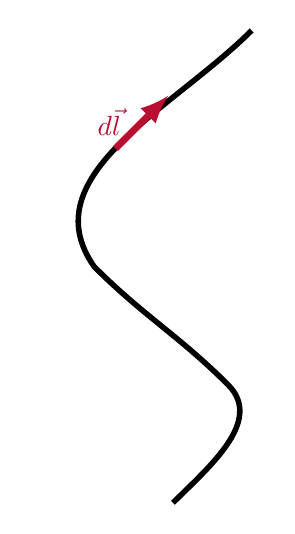
\begin{tikzpicture}[scale=1]
\scalebox{1.0}{
  \draw[line width=2pt] (0,0) to [out=45, in=-45] (0.7,1.5) to [out=135, in=-45] (-1,3) to[out=125,in=225] (1,6);
  \draw[-latex, color=qred, line width =2.5pt] (-0.73,4.5) -- +(45:0.95) node[midway, left=3pt] {$d\vec l$};

}
\end{tikzpicture}
\captionof*{figure}{\textit{The vector $d\vec l$ points in the same direction as the current.}}
}

%%%%%%%%%%%%%%%%%%%%%%%%
\subsection{Force on a curved wire}
\label{subsec:forceonacurvedwire}
\twocolframesf{Force on a curved wire}
{%
\begin{itemize}%
\item<1-> Want to know total force on the wire. %
\item<2-> The forces from the straight sections cancel.%
\item<3-> Choose a segment, of length $dl=R d\phi$, it will experience a force:%
\begin{align*}%
d\vec F = I d\vec l \times B=IBR d\phi(-\cos\phi\hat x+\sin\phi\hat y)%
\end{align*}%
\item<4-> The $x$ components of force cancel by symmetry. The total force in $y$:%
\begin{align*}%
F_y=\int_0^{\pi} IB R\sin\phi d\phi=IBR%
\end{align*}%
\end{itemize}%
\vspace{-0.2cm}
\only<4>{\emph{You can easily convince yourself that the net force on a closed circular loop is zero!}
}}
{
\centering
\begin{tikzpicture}[scale=1]
\def\R{2}
\def\L{2}
\def\F{0.5*\R}
\def\Fx{\F*0.766}
\def\Fy{\F*0.643}
\def\RF{1.4*\R}
\def\LF{1.4*\L}

\def\Nbx{10}
\def\Nby{8}

\draw[line width = 1.5pt] (-\R,-\L) -- (-\R,0) arc (180:0:\R) -- (\R,-\L);
\draw[line width = 1.5pt, -latex] (-\R,-0.75\L) -- (-\R,-0.25*\L) node[midway,left]{$I$};
\draw[line width = 1.5pt, -latex] (\R,-0.25*\L) -- (\R,-0.75\L)  node[midway,right]{$I$};


%%B field

\foreach \i in {1,...,\Nbx}{
  \def\xi{-\RF - \RF/\Nbx + \i*2*\RF/\Nbx}
  \foreach \j in {1,...,\Nby}{
    \def\yj{-\LF - \LF/\Nby + \j*2*\LF/\Nby}
    \node[color=qblue!70, opacity=0.8] at (\xi,\yj) {$\times$};
  }
}

%origin
\fill (0,0) circle (2pt);

%lines
\draw [dashed] (-\R,0) -- (\R,0);
\draw [latex-latex] (-0.9*\R,-\L) -- (-0.9*\R,0) node[midway, right] {$l$};
\draw [-latex,dashed] (0,0) -- (140:\R) node[midway, left] {$R$};

%labels
\node[above=12pt,color=qblue!70,] at (0,-\LF) {$\vec B$};

\only<3->{
%constructions for the math
\draw[-latex, color=qred, line width=0.6pt] (180:0.35*\R) arc (180:140:0.35*\R) node [midway,left] {$\phi$};
\draw[-latex, color=qred, line width = 1.5pt] (140:\R) -- (125:\R) node [right=3pt] {$d\vec l$};
\draw [dashed, color=qred] (0,0) -- (125:\R);
\draw[color=qred, line width=1pt] (140:0.45*\R) arc (140:125:0.45*\R) node [midway,right] {$d\phi$};

%left side
\draw [-latex,line width = 2, color=qblue] (140:\R)--(140:\R+\F) node[above] {$d\vec F$};
\draw [line width = 1, color=qblue, dashed] (140:\R) -- ($(140:\R)+(-\Fx,0)$) node[below=8pt,right=-2pt] {$dF_x$};
\draw [line width = 1, color=qblue, dashed] (140:\R+\F) -- ($(140:\R+\F)+(0,-\Fy)$) node[midway, left] {$dF_y$};
}

\only<4->{
%right side
\draw [-latex,line width = 2, color=qblue] (40:\R)--(40:\R+\F) node[above] {$d\vec F$};
\draw [line width = 1, color=qblue, dashed] (40:\R) -- ($(40:\R)+(+\Fx,0)$) node[below=8pt,left=-2pt] {$dF_x$};
\draw [line width = 1, color=qblue, dashed] (40:\R+\F) -- ($(40:\R+\F)+(0,-\Fy)$) node[midway, right] {$dF_y$};
\draw [dashed] (0,0) -- (40:\R);
\draw[-latex, color=qred, line width=0.6pt] (0:0.35*\R) arc (0:40:0.35*\R) node [midway,left] {$\phi$};
}


\end{tikzpicture}
\captionof*{figure}{\textit{A curved current-carrying wire in a magnetic field.}}
}



%%%%%%%%%%%%%%%%%%%%%%%%%%




%%%%%%%%%%%%%%%%%%%%%%%%%%%%%%




%%%%%%%%%%%%%%%%%%%%%%%%%%%%




%%%%%%%%%%%%%%%%%%%%%%%%%




%%%%%%%%%%%%%%%%%%%%%%%%%





%%%%%%%%%%%%%%%%%%%%%%%%%%
\end{document}

